\documentclass[a5paper]{article}
\usepackage[a5paper, top=8mm, bottom=8mm, left=8mm, right=8mm]{geometry}

\usepackage{polyglossia}
\setdefaultlanguage[babelshorthands=true]{russian}

\usepackage{fontspec}
\setmainfont{FreeSerif}
\newfontfamily{\russianfonttt}[Scale=0.7]{DejaVuSansMono}

\usepackage[font=scriptsize]{caption}

\usepackage{amsmath}
\usepackage{amssymb,amsfonts,textcomp}
\usepackage{color}
\usepackage{array}
\usepackage{hhline}
\usepackage{cite}

\usepackage[hang,multiple]{footmisc}
\renewcommand{\footnotelayout}{\raggedright}

\PassOptionsToPackage{hyphens}{url}\usepackage[xetex,linktocpage=true,plainpages=false,pdfpagelabels=false]{hyperref}
\hypersetup{colorlinks=true, linkcolor=blue, citecolor=blue, filecolor=blue, urlcolor=blue, pdftitle=1, pdfauthor=, pdfsubject=, pdfkeywords=}

\usepackage{tabu}

\usepackage{graphicx}
\usepackage{indentfirst}
\usepackage{multirow}
\usepackage{subfig}
\usepackage{footnote}
\usepackage{minted}

\sloppy
\pagestyle{plain}

\title{Примеры архитектур}

\date{}

\begin{document}

\maketitle
\thispagestyle{empty}

\section{Введение}

Начать имеет смысл с первоисточников, по которым подготовлена эта лекция:
\begin{itemize}
	\item краткий обзор архитектуры Git в <<The Architecture of Open Source Applications>>\footnote{\url{http://aosabook.org/en/git.html}} и, что полезнее, но длиннее, глава 10 Git Book\footnote{\url{https://git-scm.com/book}};
	\item обзор архитектуры Mercurial в той же <<The Architecture of Open Source Applications>>\footnote{\url{http://aosabook.org/en/mercurial.html}}, и, как обычно, документация\footnote{\url{http://hgbook.red-bean.com/read/}};
	\item книжка по SVN\footnote{\url{http://svnbook.red-bean.com/}}, в AOSA они написать поленились.
\end{itemize}

Для того, чтобы рассказывать про системы контроля версий, имеет смысл сначала пояснить, откуда они вообще появились, как развивались и к чему пришли. Вообще, то, что надо как-то хранить исходники, управлять изменениями в них и координировать действия разработчиков, стало очевидным практически сразу же, но пока исходники хранились на перфокартах, это не было особой проблемой.

Первые системы контроля версий были централизованными, что, в общем-то, неудивительно. Первая специализированная система контроля версий называлась SCCS (Source Code Control System) и появилась примерно в 1975 году. Она ничего не умела, кроме как хранить версии в виде дельт, что было более эффективно, чем просто раскладывать исходники по папкам (для тогдашних носителей информации даже текстовые исходники были серьёзной нагрузкой). В 1982 году появилась RCS (Revision Control System), которая была несколько более продвинутой и, главное, опенсорсной\footnote{\url{https://www.gnu.org/software/rcs/}} (и, что интересно, до сих пор поддерживается GNU --- неизвестно насколько <<до сих пор>>, актуальная версия, 5.9.4, вышла в 2015 году, но между 5.7 и 5.8 прошло 16 лет, так что это не показатель. GNU-ваариант SCSS\footnote{\url{https://www.gnu.org/software/cssc/}}, переписанная с нуля SCSS, тоже до сих пор поддерживается и даже более жив, версия 1.4.1 вышла в 2019-м; что характерно, оба проекта хранят исходники в git).

Первая система, которая по-настоящему поддерживала более-менее автоматизированные мерджи, была CVS (1986 год). Там же впервые появились понятия <<ветка>> и <<тэг>>. Поначалу CVS использовала сетевую шару для хранения репозитория, но потом даже была реализована клиент-серверная архитектура, как у современных систем контроля версий. Дальнейшее развитие идей CVS --- система Subversion, 2000 год. Subversion в качестве единицы версионирования использовала (использует! Subversion жива до сих пор) целое дерево исходников, так что там были глобальные для репозитория версии с целочисленными номерами, которые постепенно увеличивались. Кроме того, Subversion локально хранила и рабочую копию, и последнюю немодифицированную версию исходников, что позволяло дифф с последней версией выполнять локально, а значит, быстро. Ещё в Subversion интересно то, что ветки и тэги --- это не какие-то специальные сущности, а просто папки с исходниками в общем репозитории. Поэтому автоматический импорт репозитория из Subversion в git честно выкладывал все ветки в одну, так что в мастере оказывалась куча несколько отличающихся версий проекта. У меня у самого был как-то коммит, удалявший более миллиона строк кода из проекта, где их в то время было всего 120 тысяч, как раз удаление старых веток, импортированных из Subversion.

Отдельного упоминатия заслуживает Microsoft Visual SourceSafe (VSS), 1994 год. Он помер в 2005-м, но активно использовался в индустрии даже несколько после прекращения сопровождения. Поначалу был чисто локальным, потом научился работать через сетевую шару, а в последней версии (в 2005 году!) научился клиент-серверной работе. Поскольку с автоматическими мерджами там было не очень, он предпочитал использовать подход эксклюзивного редактирвоания файлов --- разработчик, желающий что-то поменять, берёт замок на файл, редактирует, выкладывает файл и снимает замок. Это жизнеспособно для больших проектов с не очень большими командами, где мала вероятность одновременной модификации одного файла, но вообще это, конечно, ад. Имел несчастье работать с этой штукой.

В 2005 году начали массово появляться распределённые системы контроля версий, с быстрой и удобной реализацией веток и мерджей. О двух таких системах --- Git и Mercurial --- и пойдёт речь в этой лекции. Из прочих популярных систем останутся за кадром распределённый GNU Bazaar (тоже 2005 год), централизованный проприетарный Microsoft Team Foundation Server (TFS, тоже 2005 год!), ныне известный как Azure DevOps Server (хотя технически это не система контроля версий, а система управления проектом наподобие GitLab, правильнее говорить <<Team Foundation Version Control>>). TFS очень популярен ныне в .NET-мире, хотя поначалу тоже, как VSS, реализовывал страшную схему с эксклюзивным редактированием файла (причём, файлы в рабочей копии были read-only). Очень быстро его научили неэксклюзивной работе, с мерджами, но коммиты всё ещё делаются на центральный сервер.

\section{Git}

\subsection{Ключевые требования}

Git, как известно, распределённая система контроля версий, поэтому весь репозиторий вынужден хранить локально. Появился он в результате грустной истории с ядром Linux --- оно некоторое время хранилось в проприетарной распределённой системе BitKeeper (2000 год, кстати, одна из первых), но потом разработчики ядра что-то не поделили с компанией-производителем (BitMover), и им пригрозили отзывом лицензии. Линусу Торвальдсу пришлось срочно разрабатывать новую систему контроля версий (потому что ему не нравилась система CVS, в которой так же хранились исходники Linux в то время). Поначалу это был просто набор скриптов на bash для управления патчами, приходившими по почте. С самого начала основными требованиями к разработке были следующие.

\begin{itemize}
	\item Распределённая разработка с тысячей коммитеров --- так же, как в BitKeeper и не так, как в CVS, должны были быть поддержаны процессы, при которых каждый участники может работать у себя локально, не мешая ничьей работе и сам определяя, когда его часть готова к публикации. Для большого проекта с открытым исходным кодом, надо которым работают тысячи никому ничего не должных энтузиастов, это необжодимо.
	\item Защита от порчи исходников --- возможность отменить мердж, смерджиться вручную. Опять-таки, тысячи энтузиастов, которые никому ничего не должны, и половина из которых вообще толком программировать не умеет.
	\item Высокая скорость работы --- речь идёт о сотнях тысяч коммитов всё-таки.
\end{itemize}

Несколько иронично то, что BitKeeper сам в 2016 году стал опенсорсным, и при этом не то чтобы очень популярен. Никогда не ссорьтесь с opensource-сообществом по поводу лицензий на ПО.

\subsection{Представление репозитория}

Когда мы набираем \mintinline{text}|git init|, создаётся папка \mintinline{text}|.git|, где лежит вся информация гитового репозитория. Она имеет следующую структуру:

\begin{itemize}
	\item \textbf{HEAD} --- ссылка на текущую ветку, которую зачекаутили в рабочей папке;
	\item \textbf{index} --- staging area, то место, где формируется информация о текущем коммите;
	\item \textbf{config} --- конфигурационные опции гита для этого репозитория;
	\item \textbf{description} --- <<is only used by the GitWeb program, so don’t worry about it>> (c) Git Book;
	\item \textbf{hooks/} --- хук-скрипты (возможность исполнить произвольный код при каком-то действии типа коммита), про которые мы сейчас не будем и в домашке их поддерживать не надо;
	\item \textbf{info/} --- тоже локальные настройки репозитория, сюда можно вписать игнорируемые файлы, которые вы не хотите писать в .gitignore, чтобы их не коммитить;
	\item \textbf{objects/} --- самое интересное, тут лежит собственно то, что хранится в репозитории;
	\item \textbf{refs/} --- тут лежат указатели на объекты из objects (ветки, как мы увидим в дальнейшем);
	\item \textbf{...} --- прочие штуки, которые появляются в процессе жизни репозитория и нам пока не интересны.
\end{itemize}

Гит вообще появился как набор утилит, которые позволяют быстро сделать систему контроля версий, а не как полноценная система контроля версий, так что у гита, помимо общеизвестных команд, есть и команды, позволяющие напрямую работать с репозиторием и делать с ним вручную ужасные вещи. Сам по себе репозиторий в гите --- это просто хеш-таблица, которая отображает SHA-1-хеш файла в содержимое файла, ничего более. Можно класть в неё объекты (даже не обязательно файлы), можно получать. Например, вот так:

\begin{minted}{bash}
$ git init test
Initialized empty Git repository in /tmp/test/.git/
$ cd test
$ find .git/objects
.git/objects
.git/objects/info
.git/objects/pack

$ echo 'test content' | git hash-object -w --stdin
d670460b4b4aece5915caf5c68d12f560a9fe3e4

$ find .git/objects -type f
.git/objects/d6/70460b4b4aece5915caf5c68d12f560a9fe3e4
\end{minted}

Создали пустой репозиторий, гит нам создал структуру папок \mintinline{bash}|.git/objects|, пока пустую. Командой \mintinline{text}|git hash-object| мы положили в репозиторий новый объект --- строчку \mintinline{bash}|'test content'|. Ключ \mintinline{bash}|-w| означает, что надо не просто посчитать хеш объекта, но и реально записать его на диск, ключ \mintinline{bash}|--stdin| означает, что содержимое объекта надо получить из входного потока, а не из файла. Вызов этой команды вернул нам SHA-1-хеш того, что получилось, и заодно создал файл на диске с содержимым, положив его в \mintinline{bash}|.git/objects|, в подпапку, называющуюся как первые два символа хеша, и в файл, называющийся как остальные 38 символов хеша.

Как достать то, что мы сохранили, обратно:
\begin{minted}{text}
$ git cat-file -p d670460b4b4aece5915caf5c68d12f560a9fe3e4
test content
\end{minted}

Команда \mintinline{bash}|git cat-file| показывает содержимое файла, ключ \mintinline{bash}|-p| говорит определить тип объекта и красиво показать его содержимое.

Уже можно сделать версионный контроль вручную с использованием рассмотренных команд (правда, для этого нам потребуется настоящий файл, версионировать строку, как в предыдущем примере, не интересно):

\begin{minted}{bash}
$ echo 'version 1' > test.txt
$ git hash-object -w test.txt
83baae61804e65cc73a7201a7252750c76066a30

$ echo 'version 2' > test.txt
$ git hash-object -w test.txt
1f7a7a472abf3dd9643fd615f6da379c4acb3e3a

$ find .git/objects -type f
.git/objects/1f/7a7a472abf3dd9643fd615f6da379c4acb3e3a
.git/objects/83/baae61804e65cc73a7201a7252750c76066a30
.git/objects/d6/70460b4b4aece5915caf5c68d12f560a9fe3e4

$ git cat-file -p 83baae61804e65cc73a7201a7252750c76066a30 > test.txt
$ cat test.txt
version 1

$ git cat-file -p 1f7a7a472abf3dd9643fd615f6da379c4acb3e3a > test.txt
$ cat test.txt
version 2
\end{minted}

Каждая новая версия в данном случае хранится как отдельный объект, но всему своё время.

Объект, кстати, называется <<blob>> (Binary Large OBject), и он хранит только данные, так что даже имя файла в нём не хранится, а, наверное, хотелось бы. За хранение имени файла, а также за хранение папок и вообще иерархии объектов отвечает объект <<tree>>. Например, вот так могло бы выглядеть дерево, на которое указывает коммит \mintinline{text}|master| в некотором репозитории (два файла и одно поддерево):

\begin{minted}{text}
$ git cat-file -p master^{tree}
100644 blob a906cb2a4a904a152e80877d4088654daad0c859      README
100644 blob 8f94139338f9404f26296befa88755fc2598c289      Rakefile
040000 tree 99f1a6d12cb4b6f19c8655fca46c3ecf317074e0      lib
\end{minted}

Синтаксис \mintinline{text}|master^{tree}| говорит, что надо отобразить master как tree-объект, а не как commit-объект. Вот так можно себе представить дерево, приведённое в примере:

\begin{center}
	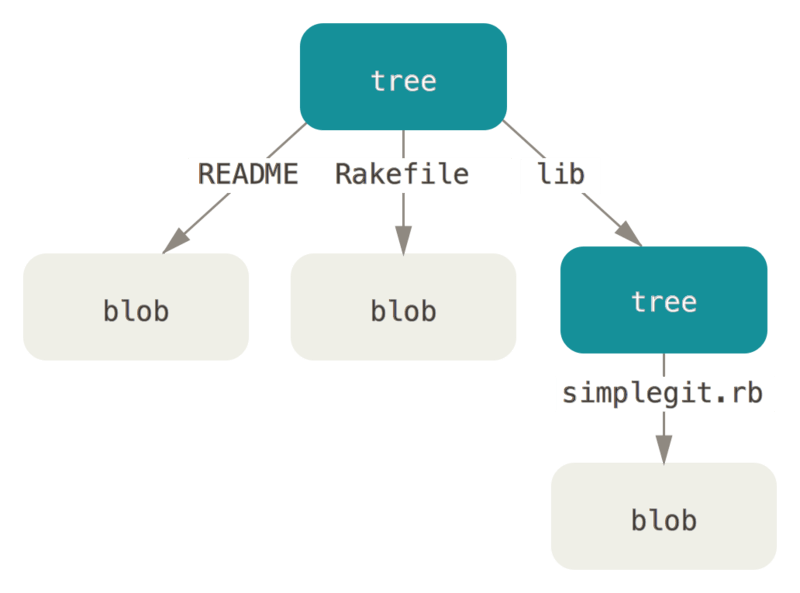
\includegraphics[width=0.5\textwidth]{gitTreeObject.png}
\end{center}

Вот примерная UML-диаграмма классов всех объектов, которые могут находиться в гитовом репозитории:
\begin{center}
	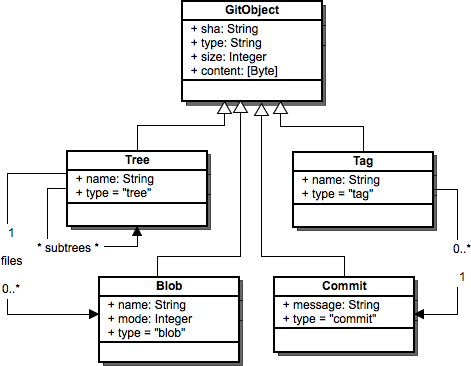
\includegraphics[width=0.7\textwidth]{gitDataStructure.png}
\end{center}

Все они являются объектами, поэтому имеют свой SHA-1-хеш, тип, который позволяет их отличить друг от друга, размер и данные. Blob и Tree мы уже видели, Tree содержит в себе поддеревья и Blob-ы. Осталось разобраться с коммитами и тэгами. 

Коммиты нужны для хранения метаинформации --- кто сделал изменение, когда и почему. Дерево ничего такого не хранит, в этом смысле оно напоминает узел файловой системы (в UNIX-подобных системах распространён термин inode), так что на объекты из дерева ссылаются коммит-объекты. Вот так это выглядит:
\begin{minted}{text}
$ echo 'first commit' | git commit-tree d8329f
fdf4fc3344e67ab068f836878b6c4951e3b15f3d

$ git cat-file -p fdf4fc3
tree d8329fc1cc938780ffdd9f94e0d364e0ea74f579
author Scott Chacon <schacon@gmail.com> 1243040974 -0700
committer Scott Chacon <schacon@gmail.com> 1243040974 -0700

first commit
\end{minted}

Ещё, что не показано на картинке, но тоже есть --- коммит хранит список коммитов-родителей, но вообще понятие <<родитель>> для коммита связано с ветками, поэтому про них чуть попозже. Вот, наверное, знакомая картинка про то, как коммиты можно представлять себе в виде указателей на узлы дерева в базе:

\begin{center}
	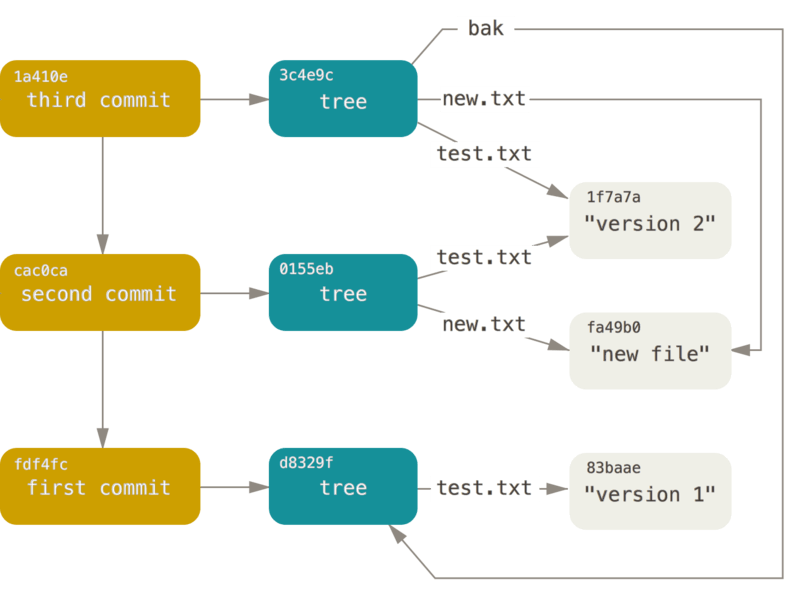
\includegraphics[width=0.7\textwidth]{gitCommitObjects.png}
\end{center}

Теперь у нас есть объекты, хранящие в себе содержимое файлов (blob-ы), объекты, хранящие в себе структуру файлов и их имена (tree-объекты), объекты, хранящие в себе информацию об истории модификаций первых двух видов объектов, и уже, в принципе, система контроля версий могла бы получиться. Но пользоваться ей было бы очень неудобно, потому что каждый объект идентифицируется только своим SHA-1-хешем, и чтобы делать что-нибудь содержательное, надо было бы эти хеши помнить. Чтобы с этим помочь, придуманы references. Reference --- это просто ссылка на коммит. Reference даже не объект, это просто файл, внутри которого лежит SHA-1-хеш объекта из базы. При этом reference-ы бывают двух типов --- head-ы и tag-и. Они хранятся в папке \mintinline{text}|.git/refs|, \mintinline{text}|.git/refs/heads| и \mintinline{text}|.git/refs/tags| соответственно. Мы можем сделать свою собственную ветку, создав сами такой файл:

\begin{minted}{text}
$ echo "1a410efbd13591db07496601ebc7a059dd55cfe9" > .git/refs/heads/master

$ git log --pretty=oneline master
1a410efbd13591db07496601ebc7a059dd55cfe9 third commit
cac0cab538b970a37ea1e769cbbde608743bc96d second commit
fdf4fc3344e67ab068f836878b6c4951e3b15f3d first commit
\end{minted}

Совсем вручную это делать можно, но не принято, есть команда \verb|git update-ref|, которая, во-первых, проверяет, что ref создаётся в правильной папке, во-вторых, заносит действие с reference в так называемый reflog, про который тоже чуть попозже, но вообще --- это штука, которая помнит, что происходило со ссылками и может помочь востановить случайно удалённую ветку. Традиционная картинка, поясняющая суть ссылок:

\begin{center}
	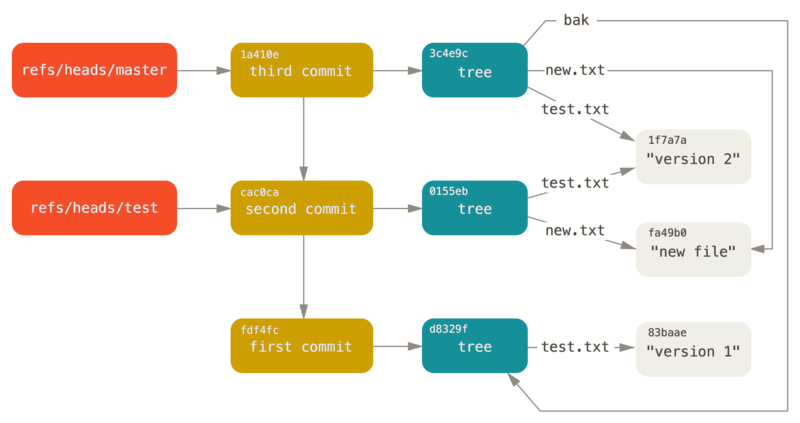
\includegraphics[width=0.9\textwidth]{gitRefs.png}
\end{center}

Среди всех ссылок выделяется самая главная, та, которая соответствует ветке, лежащей сейчас в рабочей копии. Она внезапно хранится не в \mintinline{text}|.git/refs|, а прямо в корне папки \mintinline{text}|.git|, в файле, который называется \mintinline{text}|HEAD|. Причём это даже не ссылка, а символическая ссылка, то есть ссылка на ссылку:

\begin{minted}{text}
$ cat .git/HEAD
ref: refs/heads/master

$ git symbolic-ref HEAD refs/heads/test
$ cat .git/HEAD
ref: refs/heads/test
\end{minted}

Команда \mintinline{text}|git symbolic-ref| нужна для <<вежливого>> обновления символической ссылки, которая проверяет корректность того, что происходит. Таким нехитрым образом можно переключаться между ветками, но обратите внимание, что \mintinline{text}|index| ничего про это не знает, так что файлы из старой ветки будут считаться добавленными к коммиту, потому что они были в её индексе и никто их оттуда не убрал. Так что \mintinline{text}|git checkout| всё-таки не только обновляет HEAD.

Последний из объектов, который надо рассмотреть --- это тэги. Тэг --- это просто указатель на коммит. Ну, на самом деле, не всё так просто, потому что мы видели его на диаграмме с объектами в базе, а reference --- не объект. Дело в том, что тэги бывают двух типов --- легковесные и аннотированные. Легковесный тэг --- это просто ссылка на коммит, которая никогда никем не двигается (её можно продвинуть вручную, но это плохо, поскольку тогда у людей, имеющих копии вашего репозитория, тэги могут начать не совпадать). Аннотированный тэг --- это уже полноценный объект, который указывает на коммит, и нужен он для того, чтобы иметь возможность добавить к тэгу разную метаинформацию типа автора, сообщения и даты.

Пример, как сделать вручную легковесный тэг:
\begin{minted}{text}
git update-ref refs/tags/v1.0 cac0cab538b970a37ea1e769cbbde608743bc96d
\end{minted}

А вот аннотированный тэг и как он хранится:
\begin{minted}{text}
$ git tag -a v1.1 1a410efbd13591db07496601ebc7a059dd55cfe9 -m 'test tag'

$ git cat-file -p 9585191f37f7b0fb9444f35a9bf50de191beadc2
object 1a410efbd13591db07496601ebc7a059dd55cfe9
type commit
tag v1.1
tagger Scott Chacon <schacon@gmail.com> Sat May 23 16:48:58 2009 -0700

test tag
\end{minted}

\subsection{Pack-файлы}

Казалось бы, теперь всё, но тут мы вспоминаем, что все объекты в репозитории всё ещё хранятся целиком, так что если у нас есть длиннющий исходник и мы в нём поменяли одну строчку, у нас получится два длиннющих исходника. Самое удивительное, что, в общем-то, в гите поначалу так и есть, репозиторий некоторое время просто раскопирует изменённые файлы. Естественно, файлы сжимаются zlib-ом, так что занимают чуть меньше места, чем могли бы, но всё равно, для системы контроля версий такая ситуация довольно странна. На помощь приходят pack-файлы:

\begin{minted}{text}
$ git gc
Counting objects: 18, done.
Delta compression using up to 8 threads.
Compressing objects: 100% (14/14), done.
Writing objects: 100% (18/18), done.
Total 18 (delta 3), reused 0 (delta 0)

$ find .git/objects -type f
.git/objects/bd/9dbf5aae1a3862dd1526723246b20206e5fc37
.git/objects/d6/70460b4b4aece5915caf5c68d12f560a9fe3e4
.git/objects/info/packs
.git/objects/pack/pack-978e03944f5c581011e6998cd0e9e30000905586.idx
.git/objects/pack/pack-978e03944f5c581011e6998cd0e9e30000905586.pack
\end{minted}

Тут мы выполнили команду \mintinline{text}|git gc| (Garbage Collect), в результате которой некоторые <<нормальные>> объекты удалились (на самом деле, все кроме <<висячих>>, то есть недостижимых по ссылкам) и появилось два файла: \mintinline{text}|.idx| и \mintinline{text}|.pack|. Второй файл содерхит упакованными все наши объекты, и тут уже применяется дельта-компрессия, причём, что интересно, последняя версия файла хранится целиком, а предыдущие версии --- как дельты относительно более свежей версии, то есть как бы <<назад>> (что логично, скорее всего, последняя версия нужна чаще). Первый файл --- это оглавление для второго файла, именно его передают по сети, когда делается git push/git pull и локальный или удалённый гит пытается понять, какой информации у него нету. Вот так примерно это выглядит:

\begin{center}
	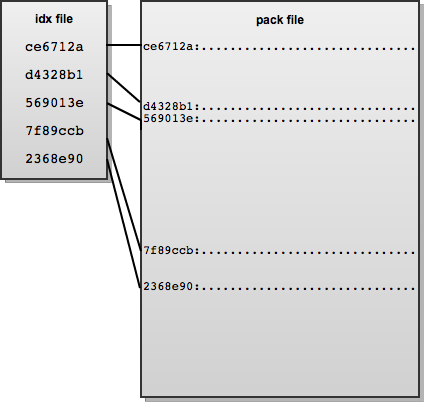
\includegraphics[width=0.6\textwidth]{gitPackFiles.png}
\end{center}

Упаковка объектов в .pack-файлы происходит, когда:
\begin{itemize}
	\item Выполняется git push;
	\item Слишком много <<свободных>> объектов (порядка 7000);
	\item Вручную вызвана git gc.
\end{itemize}

Если pack-файл уже есть, то новые объекты могут упаковаться в новый файл, оставив старый неизменённым, а может произойти перепаковка и несколько .pack-файлов будут слиты в один (важно понимать, что .pack-файлов может быть несколько и вся работа с ними скрыта от пользователя системы контроля версий). Почему всё так хитро --- упаковка в .pack-файл требует пересчёта дельт и вообще очень трудоёмкая операция, так что делать её каждый коммит было бы очень раздражающе для пользователя. Есть ещё команда \mintinline{text}|git gc --auto|, которая проверяет, не надо ли запаковать объекты, она вызывается при каждом коммите и, как правило, ничего не делает, иногда всё-таки вызывая \mintinline{text}|git gc|. Внутрь pack-файла можно посмотреть командой \mintinline{text}|git verify-pack|, не то чтобы сильно полезно на практике, так что подробности в Git Book.

\subsection{Reflog}

Все нормальные команды гита записывают всё, что они делали с reference-ами в файлы в папке \mintinline{text}|logs|, где, в частности, лежит лог того, что происходило со ссылкой \mintinline{text}|HEAD|, и его можно просмотреть командой \mintinline{text}|git reflog|:

\begin{minted}{text}
$ git reflog
1a410ef HEAD@{0}: reset: moving to 1a410ef
ab1afef HEAD@{1}: commit: modified repo.rb a bit
484a592 HEAD@{2}: commit: added repo.rb
\end{minted}

Или получить более подробную информацию командой \mintinline{text}|git log -g|:

\begin{minted}{text}
$ git log -g
commit 1a410efbd13591db07496601ebc7a059dd55cfe9
Reflog: HEAD@{0} (Scott Chacon <schacon@gmail.com>)
Reflog message: updating HEAD
Author: Scott Chacon <schacon@gmail.com>
Date:   Fri May 22 18:22:37 2009 -0700

    third commit
$ git branch recover-branch ab1afef
\end{minted}

Если мы случайно откатили ветку и потеряли тем самым какой-то нужный коммит, можно найти его в reflog-е, взять его хеш и сделать на него checkout.

А теперь как более капитально прострелить себе ногу. Шаг 1, удаляем ветку:

\begin{minted}{text}
$ git branch -D master
\end{minted}

Шаг второй, сносим все логи, чтобы нельзя было восстановить ветку по SHA-1-хешу последнего коммита, на который она указывала:

\begin{minted}{text}
$ rm -Rf .git/logs/
\end{minted}

Казалось бы, всё, репозиторий запорот и надо делать домашку заново? Нет, если база объектов на месте, можно воспользоваться командой \mintinline{text}|git fsck --full|, которая распечатает нам все висячие объекты вместе с их хешами:

\begin{minted}{text}
$ git fsck --full
Checking object directories: 100% (256/256), done.
Checking objects: 100% (18/18), done.
dangling blob d670460b4b4aece5915caf5c68d12f560a9fe3e4
dangling commit ab1afef80fac8e34258ff41fc1b867c702daa24b
dangling tree aea790b9a58f6cf6f2804eeac9f0abbe9631e4c9
dangling blob 7108f7ecb345ee9d0084193f147cdad4d2998293
\end{minted}

Теперь мы можем посмотреть на них командой \mintinline{text}|git cat-file -p|, выбрать тот, который больше всего похож на последний коммит той ветки, которую мы удалили, и восстановить ветку по его хешу: \mintinline{text}|git branch recover-branch ab1afef|. Ещё позитивно то, что Git не удалит даже <<висячие>> объекты несколько месяцев, если его явно не попросить, несмотря на то, как расшифровывается имя команды \mintinline{text}|git gc|, так что если вы потеряли ветку, то с большой вероятностью она всё ещё где-то есть и её можно восстановить.

\subsection{Lessons learned}

Поначалу некоторые команды были реализованы как шелл-скрипты, потому что так было быстрее. Однако это помешало, во-первых, интеграцию git со средами разработки, во-вторых, существенно усложнило портирование git на Windows. Что, в общем-то, не сильно расстроило Линуса Торвальдса и окологитовое сообщество середины 2000-х, но на самом деле негативно сказалось на внедрении git, поскольку крупные компании избегали пользоваться им из-за проблем с переносимостью. Впоследствии был реализован проект Git for Windows, где уже вся функциональность была реализована в виде разделяемой библиотеки, и дело пошло.

Ещё важный момент, проистекающий из изначального дизайна git как набора инструментов для управления патчами --- у него весьма хитрая система команд (<<plumbing>>, которым, в общем-то, никто не пользуется, и <<porcelain>>). Даже если не задумываться о том, что новички в git могут случайно нагуглить git cat-file и нескоро понять, что эти команды им знать не надо, набор команд сложноват и не то чтобы дружественен к начинающим пользователям. На первом курсе, чтобы научить студентов пользоваться git, требуется обычно две пары, плюс у них всё равно весь первый курс время от времени возникают проблемы, требующие некоторого вмешательства.

\section{Mercurial}

\subsection{Основные требования}

Разработка Mercurial началась также как следствие отказа от BitKeeper как средства версионирования ядра Linux, в 2005 году, но другим ключевым разработчиком ядра: Matt Mackall. В несколько более спокойной обстановке --- Линус Торвальдс взял на себя задачу обеспечить непрерывность процесса поддержки ядра со своим git, так что у Мэта Мэкола было время спроектировать систему контроля версий более аккуратно. В отличие от git, Mercurial проектировался как простая в использовании и при этом эффективная система контроля версий для работы с большими проектами: миллионы коммитов, миллионы файлов, десятилетия разработки и много тысяч контрибьюторов (например, ядро Linux). При этом на эффективность в большей степени влияла пропускная способность сети и скорость поиска на диске (в 2005м году SSD-диски уже были, но не то чтобы были широко распространены). Поэтому в дизайне системы необходимо было решить следующие вопросы.

\begin{itemize}
	\item Как хранить историю версий на диске? Конкретнее, как добиться максимальной скорости операций ввода-вывода, при этом избегая излишней нагрузки на процессор?
	\item Как эффективно получать предыдущие версии, даже если они очень стары?
	\item Как эффективно добавлять новые версии, не модифицируя уже существующие?
	\item Как эффективно получать историю для конкретного файла? Как эффективно получать историю для каждой конкретной строки файла (чтобы поддержать <<blame>>)?
\end{itemize}

\subsection{Revlog}

Revlog, или Revision Log, --- основа представления изменений в Mercurial. Состоит из двух файлов --- индекса и файла данных. Индекс состоит из записей фиксированной длины, по одной на каждую ревизию:

\begin{center}
	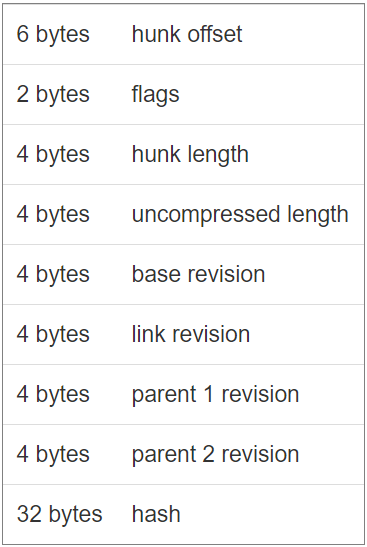
\includegraphics[width=0.3\textwidth]{revlog.png}
\end{center}

\begin{itemize}
	\item hunk offset, hunk length --- местонахождение дельты нужной нам ревизии в файле. 
	\item link revision --- ссылка на revlog более высокого уровня (про уровни чуть дальше).
	\item parent revision-ы хранятся как номера ревизий в лоокальной системе нумерации, то есть это просто числа.
	\item hash --- это глобально уникальный идентификатор ревизии, используется при работе с удалёнными репозиториями.
\end{itemize}

Фиксированность длины записи позволяет имея числовой локальный номер ревизии за константное время найти соответствующую ей запись. К тому же тот факт, что индекс хранится отдельно, позволяет нам не читать весь файл. Для хранения собственно данных применяется дельта-компрессия, но хитрая --- время от времени сохраняются чекпойнты, так что для восстановления ревизии нам надо найти ближайший чекпойнт и последовательно применить к нему дельты. При этом частота сохранения чекпойнтов определяется отношением размера предыдущего чекпойнта к суммарной длине всех дельт после него. При этом всё это ещё и жмётся zlib для пущего сокращения занимаемого объёма (как и в git).

Revlog на самом деле не один и даже не один для каждого файла, они организованы в структуру данных, позволяющую хранить информацию о ревизиях и файлах, из которых ревизия состоит, . Модель данных состоит из трёх типов revlog-ов:

\begin{itemize}
	\item changelog --- хранит метаданные всех ревизий и ссылку на manifest для каждой ревизии;
	\item manifest --- это отображение имён файлов, входящих в ревизию, в ссылки на записи для текущей ревизии в filelog-ах;
	\item filelog --- revlog для каждого файла.
\end{itemize}

Получившаяся структура изображена на рисунке:

\begin{center}
	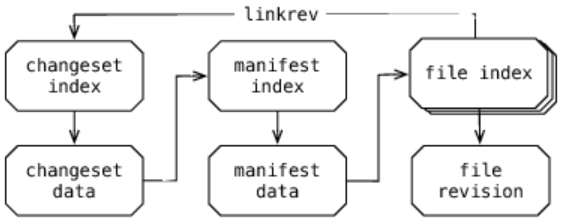
\includegraphics[width=0.5\textwidth]{mercurialLogStructure.png}
\end{center}

Внутри файлы выглядят, например, вот так. Changelog (одна ревизия):

\begin{minted}{text}
0a773e3480fe58d62dcc67bd9f7380d6403e26fa
Dirkjan Ochtman <dirkjan@ochtman.nl>
1276097267 -7200
mercurial/discovery.py
discovery: fix description line
\end{minted}

Manifest:
\begin{minted}{text}
.hgignore\x006d2dc16e96ab48b2fcca44f7e9f4b8c3289cb701
.hgsigs\x00de81f258b33189c609d299fd605e6c72182d7359
.hgtags\x00b174a4a4813ddd89c1d2f88878e05acc58263efa
CONTRIBUTORS\x007c8afb9501740a450c549b4b1f002c803c45193a
COPYING\x005ac863e17c7035f1d11828d848fb2ca450d89794
\end{minted}

Структура папок хранится прямо в манифесте --- имя файла на самом деле есть путь до файла от корня репозитория (в отличие от git, где есть специальный tree object).

Filelog-и хранятся в репозитории в папке store и называются примерно как файлы, котоырм они соответствуют (опять-таки, в отличие от git, который использует SHA-1-хеши в качестве имён файлов).

Ну и самое главное --- revlog-и жмутся дельта-компрессией (потому что собственно они-то и составляют репозиторий), поэтому, например, с точки зрения структуры данных манифест каждой ревизии содержит в себе список всех файлов в репозитории вообще, но физически на диске хранится только дельта относительно предыдущей ревизии --- то есть только изменённые файлы. Поэтому хранилище эффективно с точки зрения дискового пространства (и главное, количества потребных операций чтения), хотя и менее эффективно в плане расхода процесорного времени чем, скажем, git.

Кроме того, revlog-и при коммите обновляются в фиксированном порядке. Сначала обновляются filelog-и, затем manifest, затем уже changelog. Таким образом, если при коммите что-то пойдёт не так, changelog будет содержать в себе только корректные ссылки.

Ещё в репозитории есть dirstate --- структура данных, хранящая статус рабочей копии и ссылку на ревизию, которая является по отношению к рабочей копии базовой. dirstate используется для реализации команд status и diff, для чего она ещё и содержит кеш последнего обхода рабочей копии.

\subsection{Версии}

Версионирование в Mercurial устроено похоже на git --- ревизии организованы в дерево (точнее, дэг, потому что бывают мерджи), каждая ревизия имеет ссылку на родителя (одного или двух), номер:

\begin{center}
	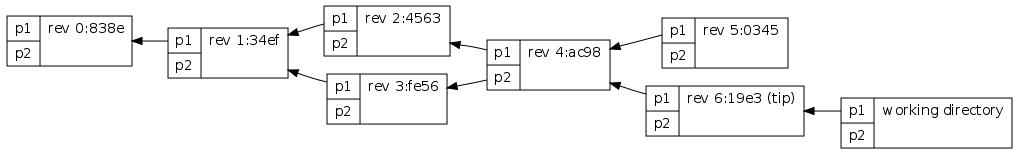
\includegraphics[width=\textwidth]{mercurialRevisions.png}
\end{center}

Важное отличие от git в том, что ревизии имеют локальный номер --- число, которое позволяет их идентифицировать в пределах одного репозитория (на одной машине). Все ссылки внутри репозитория делаются по локальным номерам, что позволяет выполнять многие операции за контантное время. Чтобы работать с удалёнными репозиториями, ревизия должна иметь кеакой-то глобально уникальный идентификатор, тут, так же, как в git, используется SHA-1-хеш содержимого ревизии.

\subsection{Ветки}

Вот ветки в Mercurial устроены необычно. Поначалу их вообще не было, чтобы сделать ветку, надо было склонить репозиторий целиком и выложить его куда-нибудь отдельно от исходного. Кажется чем-то диким, но в git есть прямой аналог --- это в fork-и на Github. Для распределённых систем контроля версий, которые без проблем могут перекладывать коммиты из репозитория в репозиторий, это вполне адекватное решение. Однако для больших проектов это оказалось не очень удобно --- клонировать весь репозиторий просто слишком дорого, как по времени, так и по месту на диске. Поэтому сделали именованные ветки: в метаданные ревизии добавили имя ветки. Что привело к интересным последствиям:

\begin{center}
	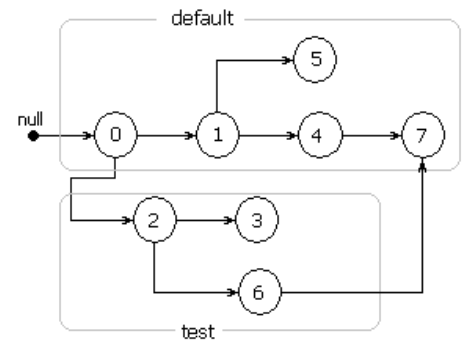
\includegraphics[width=0.5\textwidth]{mercurialBranches.png}
\end{center}

Раз имя ветки --- часть метаданных, то ничто не мешает двум ревизиям, отведёным от одного предка, относиться к одной ветке, хоть они друг с другом не связаны. Получается, что в Mercurial, в отличие от git, ветка --- это некоторый кусок дэга ревизий с общим корнем. Команда hg branch просто запоминает текущее имя ветки, а следующий коммит записывает имя ветки в данные ревизии, а по умолчанию имя ветки --- имя ветки предыдущего коммита (default сначала, как в git ветка master). А потом ещё и реализовали возможность закрыть ветку, то есть спрятать её из списка веток, добавив ещё булевый флажок в метаданные. При этом ветка могла иметь несколько head-ов --- листовых ревизий, их можно просмотреть командой hg heads. И чтобы закрыть ветку, надо было закрыть их все. Самая свежая ревизия в ветке называется <<tip>>. Кстати, ещё интересная особенность такого представления веток --- что если просто зачекаутить любую ревизию, что-то поменять и закоммитить, всё всё равно будет работать как ожидается --- создастся <<анонимная ветка>>, что очень удобно для короткоживущих веток с быстрым фиксом или попробовать что-нибудь. Не надо придумывать имя ветке, не надо её закрывать после мерджа. Git так не умеет.

Ещё есть bookmark-и --- символические ссылки на ревизии, которые работают в точности как ветки в git.

Тэги в Mercurial тоже есть, но хранятся они не как в git. Есть отдельный файл .hgtags, лежащий в корне репозитория и версионирующийся как обычный файл (примерно как обычно лежит .gitignore в git). В файле список пар из записей в changelog (их номеров) и текстовых тэгов, именующих ту или иную ревизию. Это тоже приводит к интересным последствиям --- поскольку тэги версионируются, про каждый тэг известен его автор, время, сообщение коммита. Можно ставить тэг на какую-нибудь старую ревизию. Можно без проблем поменять тэг (не как в git, где половина сокомандников забудет спуллить тэги и у всех тэги будут разными).

\subsection{Внутреннее устройство}

Mercurial написан почти целиком на Python, некоторые его части для скорости реализованы на Си. Статическая структура модулей (каждый из которых --- отдельный файл на Python или пара .c/.h) представлена на рисунке:

\begin{center}
	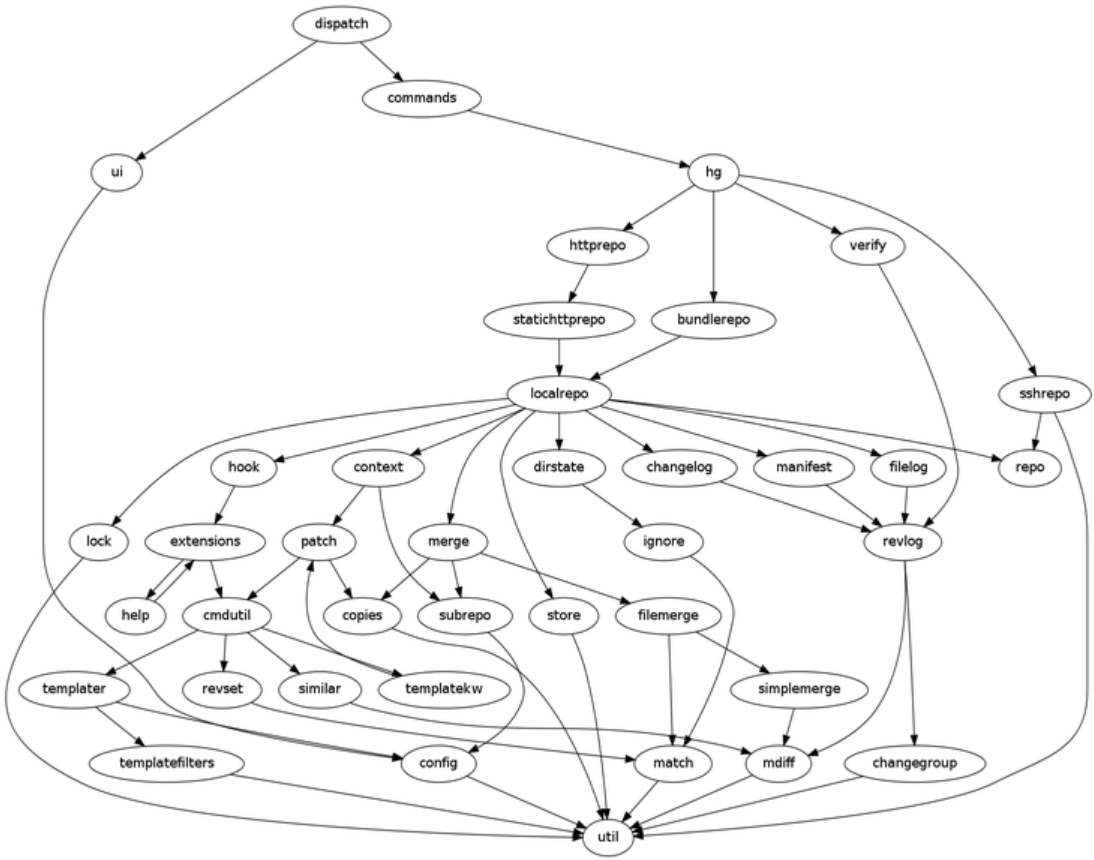
\includegraphics[width=\textwidth]{mercurialImportGraph.png}
\end{center}

Когда пользователь пишет <<hg что-то-там>>, сначала запускается модуль dispatch, который создаёт ui, который первым делом грузит конфигурацию и расширения, в ui же сохраняются глобальные опции, переданные в командной строке. Дальше смотрим на команду и понимаем, надо ли нам создать объект, представляющий локальный репозиторий (localrepo), удалённый репозиторий (httprepo, sshrepo), вообще репозиторий не нужен. Каждая команда --- это функция в модуле commands (да, один большой файл со всеми поддерживаемыми командами), там же есть хеш-табилца, которая отображает имя команды на функцию и допустимые опции командной строки. Каждая команда получает уже распарсенные опции, объект repo и ui.

\subsection{Расширяемость}

Mercurial, в отличие от git, изначально разрабатывался так, чтобы его было максимально просто расширять и затачивать под свои специфичные нужды. Предлагается сразу несколько разных точек расширения:

\begin{itemize}
	\item Новые команды -- пишем модуль расширения и добавляем туда хеш-таблицу с именем cmdtable, модуль прописываем в конфиг. При загрузке Mercurial померджит команды из своего cmdtable с командами из модуля-расширения. Также расширения могут поределить функции uisetup и reposetup, и они будут вызваны после создания объектов ui и repo, что позволяет, например, обернуть стандартынй репозиторий в свой класс-расширение и делать с ним что угодно. Например, uisetup можно использовать для того, чтобы выставлять ui.username в имя текущего залогиненного в систему пользователя.
	\item Обёртки над репозиторием --- так, например, работает hgsubversion, который представляет репозиторий Subversion так, что с ним можно работать командами Mercurial. Получается, правда, плохо, потому что Subversion --- централизованная система и не умеет в push/pull, но локально работать и коммитить вполне можно.
	\item Обёртки над любой функцией Mercurial --- можно рефлексией влезть в классы Mercurial и сделать что угодно, это ж Python. Не то чтобы это нужно делать, но разработчики вполне рассматривают этот способ как валидную точку расширения.
	\item Алиасы --- это просто новое имя для существующей команды с заранее выставленными опциями. Пишется в конфигурационном файле, не требует программирования вообще.
\end{itemize}

Ещё есть hook-и, как в git. Но в отличие от git, они бывают двух сортов --- запуск отдельных процессов или запуск Python-скриптов. Второй способ более интересен, поскольку запускается внутри процесса Mercurial (то есть быстрее, чем процесс запускать) и принимает repo и ui, что позволяет в хуке творить разные вещи. Пример использования таких хуков --- pushlog, журнал, в который записывается метаинформация о каждом пуше (чтобы потом найти и наказать виноватого).

\subsection{Lessons learned}

\begin{itemize}
	\item Python --- легко программировать, легко расширять (через хуки или точки расширения), кроме того, кроссплатформенность получилась практически даром. С другой стороны, Python медленновато работает, по крайней мере, по сравнению с Си, особенно время тратится на запуск интерпретатора, что очень печально для тулов с частыми которкими вызовами, как любая система контроля версий. Зато как язык написания расширений Python оказался очень удобен, потому что он прост. Некоторые специально учили Python, чтобы писать расширения к Mercurial.
	\item Намеренно сложно модифицировать ревизию после публикации --- есть только команда hg rollback, позволяющая откатиться только на одну ревизию. Это хорошо и правильно для выложенных куда-нибудь изменений, но плохо для изменений, которые пока сделаны локально. Что доставляет боль иногда.
	\item Revlog-и хороши и эффективны, но не дружат с переименованиями файлов.
	\item .hgtags оказался внезапен для пользователей и кого-то раздражает (тем более что в git такого нет).
	\item Небольшое количество команд якобы делает систему менее гибкой, но это считаетя основным достоинством Mercurial --- он существенно проще в изучении, чем git.
\end{itemize}

\section{Subversion}

\subsection{Основные требования}

Subversion появилась в 2000-м году как попытка заменить систему CVS в системе управления разработкой ПО CollabNet Enterprise Edition (ныне известна как TeamForge, вполне жива и продаётся до сих пор). Изначально там использовалась CVS как основное средство версионирования, с самого начала она планировалась <<на выброс>>, как только появится что-нибудь лучше. Но проблема была в том, что CVS вообще была популярна, потому что <<лучше>> просто ничего не было (по крайней мере, в open source), хотя она была жутковатой и багливой. Поэтому в CollabNet в какой-то момент приняли решение написать свою систему с нуля как замену CVS без каких-либо радикальных изменений в основных принципах, но без её багов и странных решений. CollabNet наняли Karl Fogel, известного деятеля open source, продвигавшего CVS, который по счастливой случайности как раз думал над новой системой контроля версий и уже имел на тот момент набросок архитектуры и даже имя для Subversion. И Jim Blandy, который вместе с Karl Fogel уже де-факто приступил к разработке (взяли его взаймы у Red Hat Software на неопределённый срок). К маю 2000 года была готова архитектура, в онову которой были положены следующие цели:

\begin{itemize}
	\item <<починить CVS>> --- то есть не изобретать ничего нового, а создать централизованную систему контроля версий с поддержкой клиент-серверной модели удалённого доступа;
	\item не поддерживать обратную совместимость с CVS, но сделать переход по возможности безболезненным;
	\item развивать проект как open source.
\end{itemize}

В августе 2001 исходники Subversion стали хранить в Subversion. В 2010 году проект интегрирован в Apache Software Foundation (и переименован в Apache Subversion\footnote{\url{http://subversion.apache.org}}).

\subsection{Статическая структура}

Высокоуровневая архитектура Subversion показана на рисунке\footnote{Из \url{http://svnbook.red-bean.com/en/1.7/svn-book.html\#svn.intro.architecture}}:

\begin{center}
	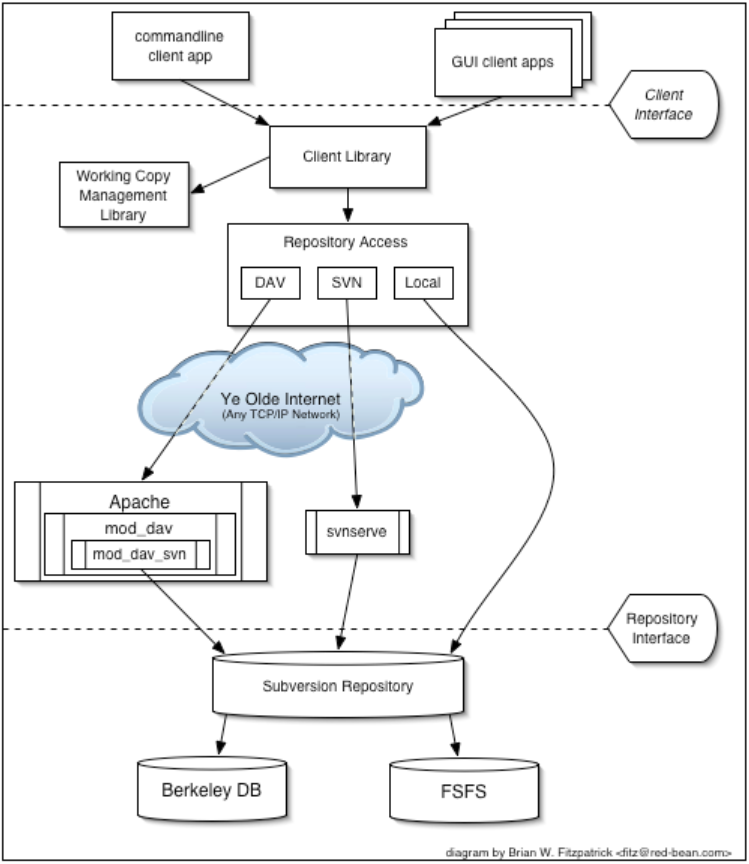
\includegraphics[width=0.7\textwidth]{subversionArchitecture.png}
\end{center}

Из интересных архитектурных решений:
\begin{itemize}
	\item репозиторий хранит ревизии в реляционной базе данных;
	\item есть Repository Access layer --- фасад для сетевой части, защищающий клиент от сложности сетевого взаимодействия;
	\item несколько разных способов ходить в репозиторий по сети;
	\item чёткое разделение на уровни.
\end{itemize}

\subsection{Ревизии, репозиторий}

Коммит в Subversion --- это просто послать слепок текущей рабочей копии на сервер. Сервер создаёт \textit{ревизию} и присваивает ей уникальный числовой номер, на один больший, чем предыдущий номер ревизии. То есть, если вы поменяли одну строчку в одном давно всеми забытом файле проекта и закоммитили, номер ревизии для всего проекта продвигается на 1. Что удобно, поскольку всегда доступен абсолютный и однозначный номер текущей версии, можно его использовать, например, в инсталляторе, чтобы собирать что-нибудь вроде MyCoolProgram1.0.0.6480.exe. Поскольку система централизованная, никаких проблем с уникальностью номера нет. Кстати, обратите внимание, в отличие от git и Mercurial, в рабочей копии сам репозиторий не хранится, там только собственно файлы исходников и немного метаинформации (в папке .svn), нужной Subversion, чтобы следить за состоянием рабочей копии и делать коммиты. Из этого следует один из главных недостатков централизованных систем --- без сетевого доступа к репозиторию почти ничего нельзя сделать, даже лог посмотреть. Коммиты в Subversion атомарны, то есть либо сервер принял набор изменений целиком, либо не принял вовсе. 

Ещё интересная особенность в том, что в рабочей копии могут быть файлы разных ревизий: допустим, вы получили версию 10, что-то поделали с файлом f.txt, зачекинили его и вам сказали, что всё ок, создана ревизия 15 (если конфликта не было, то это нормально, в отличие от git). Теперь f.txt имеет номер ревизии 15, но остальные файлы никто не обновлял (svn up ведь никто не делал, а коммит и апдейт --- архитектурно разные действия), так что они остались на ревизии 10. Это нормально и Subversion умеет с этим работать (и даже извлекать некоторую выгоду, например, вернуть заданную папку назад во времени к более старой ревизии).

Репозиторий содержит единое дерево исходников, которое обычно организовано в стандартной форме --- корневые папки trunk (<<ствол>>, основная ветка, типа master в git), branches --- ветки, и tags --- слепки trunk или веток, которые труднее поменять. Позитивно то, что если в git и Mercurial можно склонить только весь репозиторий целиком, Subversion позволяет зачекаутить только нужную папку (например, содержимое trunk, конкретной ветки, тэга или просто какую-то папку с маленьким подпроектиком, с которым вы работаете). Более того, на каждую папку можно отдельно раздавать права доступа. Репозиторий не хранит кучу копий одного файла --- если файл в нескольких разных папках один и тот же, то хранится он один раз, остальные деревья просто на него ссылаются. Так что на сервере ветки хранятся очень эффективно, в виде только изменённых файлов, зато если вы случайно зачекаутили весь репозиторий, Subversion честно размножит все файлы по папкам с ветками.

Внутри папки репозитория можно найти следующие папки:
\begin{itemize}
	\item conf/ --- папка с конфигурационными файлами
	\item db/ --- хранилище версионируемых данных. Subversion использует на выбор либо СУБД Berkley DB, либо хранение файлов в обычной файловой системе (называемое в сообществе FSFS, что-то вроде <<filesystem over filesystem>>). Berkley DB --- хранилище пар <<ключ-значение>>, наподобие современного Redis, поддерживающая транзакционность.
	\item format --- описывает организацию репозитория.
	\item hooks/ --- папка со скриптами-хуками, которые могут реагшировать на разные события в репозитории, типа появления новой ревизии.
	\item locks/ --- замки для управления одновременным доступом.
	\item README.txt --- файл, в котором просто написано, что это репозиторий Subversion.
\end{itemize}

Помимо файлов и папок в репозитории Subversion хранятся свойства --- массив пар <<ключ-значение>> для каждого элемента файловой системы (файла и папки) и для ревизий. Ключом может быть любая строка, состоящая из ASCII-шных символов, значением --- любой массив байтов. Свойства версионируются вместе с самим файлом (или папкой), кроме свойств ревизии, которые не версионируются. Часть свойств используется самой Subversion (например, \verb|svn:ignore|, \verb|svn:eol-style|), но вообще это для пользовательских скриптов, работающих с репозиторием, или для инструментов управления проектами (например, \url{https://trac.edgewall.org/}). В документации приводится хороший пример --- положим, есть у вас сайт, отображающий изображения, которых много и они часто меняются. Можно хранить изображение отдельно, описание изображения отдельно, превью уменьшенных размеров отдельно, но это неудобно, получается сильно много файлов и трудно поддерживать консистентность при частых изменениях. Subversion предлагает хранить в файловой системе только сами файлы с изображениями, а описание, дату модификации и даже уменьшенный превью хранить как свойства. И скрипт, который обновляет содержимое сайта по содержимому репозитория, может про эти своства знать, получать их простыми командами и использовать при деплое.

\subsection{Проблемы и ограничения}

У Subversion есть ряд проблем, основная из которых, пожалуй, её централизованность --- хотя это имеет и свои преимущества в виде существенно более простого жизненного цикла файлов, и, возможно, для небольших проектов с нераспределённой разработкой (домашки, НИР?) Subversion удобнее в использовании, чем git. Есть и чисто технические проблемы, которые постепенно чинятся в новых версиях\footnote{По крайней мере, по мнению \url{https://en.wikipedia.org/wiki/Apache\_Subversion}}:

\begin{itemize}
	\item Переименование файлов и папок реализовано как copy и delete. copy копирует и историю, и свойства, так что это вполне валидная реализация, но это смущает merge в случае конфликтов <<перенос-редактирование>>. В последних версиях в клиенте переименование и перенос поддержаны полноценны, но на сервере это всё ещё copy + delete.
	\item Папки .svn до версии 1.7 хранились в \textit{каждой} папке проекта, так что их содержимое находилось поиском и даже становилось жертвой рефакторингов переименования иногда. В 1.7 и выше папка .svn одна, в корне репозитория, как в других системах контроля версий.
	\item При чекауте в рабочей копии не выставляются <<настоящие>> времена модификации файлов, используется время чекаута. Это может быть неожиданно для пользователя, но это решение было осознанным --- обновлённый временной штамп заставит make и подобные утилиты пересобрать исходники после чекаута.
	\item Ветки и тэги поддержаны просто как снапшоты текущего состояния папки с проектом, никакого особого смысла для самой системы контроля версий они не несут. Что в принципе ок, поскольку репозиторий не копирует файлы, а использует символические ссылки, но вызывает некоторую конфузию у пользователей насчёт того, как организовать репозиторий. Кроме того, команды, которые логичны в git или Mercurial, в Subversion просто невозможны, например, \verb|svn log -r tag1:tag2 myfile| --- два разных тэга есть два разных снапшота файла, которые друг с другом не связаны и построить историю от одного тэга до другого без специальной инструментальной поддержки не получится.
\end{itemize}

\end{document}
